\documentclass[conference]{IEEEtran}

\usepackage{cite}
\usepackage{amsmath}
\usepackage{graphicx}
\usepackage{booktabs}
\usepackage[hyphens]{url}

% Let long URLs in the bibliography break after these characters
\def\UrlBreaks{\do\/\do-\do\.\do\_\do\=\do\?\do\&}
\Urlmuskip=0mu plus 1mu

\graphicspath{{../figures/}{figures/}}

% Rubric labels in running text
\newcommand{\lbl}[1]{\textit{#1}}
% Shell commands in running text
\newcommand{\cmd}[1]{\texttt{#1}}

\begin{document}

\title{Do LLM Red-Team Agents Generate Realistic Honeypot Traffic? A Transfer Study Against Real Cowrie Sessions}

\author{\IEEEauthorblockN{Parth Kansal and Keshav}
\IEEEauthorblockA{Affiliation TBD}}

\maketitle

\begin{abstract}
Defensive models for honeypot traffic need labeled attack sessions, and such sessions are scarce. A tempting fix is to let LLM red-team agents attack a honeypot we control and train on what they do. We tested whether this works. Three LLM attackers (DeepSeek-V3.2, Gemma-3-4B and GPT-OSS-120B) each ran 20 SSH sessions against two Cowrie honeypots. One used static shell emulation; the other took its replies from Qwen3-32B. We compared these 120 sessions with 1,672 interactive sessions from one day of the public CyberLab honeynet. Without any labels, the two corpora are far apart. On a scale from 0 to 1, the Jensen-Shannon divergence between their command-verb distributions is 0.700 (95\% CI 0.688--0.717). A simple classifier separates them with an AUC of 1.000. The gap is one of intent. The agents browsed files and hunted for credentials, while 1,038 real sessions ran the same cryptominer dropper. We labeled sessions with two blind, independent LLM annotators (Cohen's kappa 0.898). A classifier trained on the 120 synthetic sessions reached a macro-F1 of 0.205 on real sessions (0.071 on the 22 distinct real templates), against 0.983 for one trained on real sessions. Adding the synthetic sessions to the real training data gave no gain (0.981). We also found that GPT-OSS-120B pasted its own chat-format tokens and reasoning into the shell in 18 of its 40 sessions. In our setting, a single ``explore the system'' persona did not produce useful training data for real honeypot traffic.
\end{abstract}

\begin{IEEEkeywords}
Honeypots, Cowrie, large language models, synthetic data, dataset shift, intrusion detection
\end{IEEEkeywords}

%% =====================================================================
\section{Introduction}

Honeypots give defenders a direct record of what attackers do. A medium-interaction SSH honeypot such as Cowrie~\cite{oosterhof2015cowrie} logs the passwords tried, the commands typed and the files fetched. These logs can train defensive models. One example is a classifier that tags each session with its main goal, in the spirit of MITRE ATT\&CK tactics~\cite{strom2018attack}. The problem is supply. In the day of CyberLab data~\cite{sedlar2020cyberlab} that we study, only 1,672 of 76,785 sessions ran even one command. Most of those repeat a handful of bot scripts.

LLM agents look like an easy way around this shortage. Recent work shows that they can plan and run multi-step attacks~\cite{deng2024pentestgpt,fang2024hack}. If we point such an agent at a honeypot we own, it will produce sessions on demand and at low cost. Whether those sessions resemble real attacks is a separate question. LLMs carry strong ideas about what a hacker does in a capture-the-flag game. The bots that fill real honeypot logs behave differently.

We ask a narrow question. Does a classifier trained on agent-generated sessions work on real honeypot sessions, and if not, where do the two kinds of data differ? We answer in two steps. First, we measure the difference without labels. Second, we train and test classifiers on every mix of synthetic and real data, using labels from blind LLM annotation rather than keyword rules.

Our contributions are as follows.
\begin{enumerate}
\item We release an open pipeline that runs LLM attackers against Cowrie, parses the CyberLab export and regenerates every table in this paper.
\item We show, without using labels, that agent sessions are easy to tell apart from real ones and that the gap lies in attacker intent.
\item Our four-way transfer experiment shows that a classifier trained on these 120 synthetic sessions fails on real data, and that adding them to real training data gives no consistent gain.
\item We document two pipeline hazards: GPT-OSS-120B leaks chat-format tokens into the shell, and a standard Cowrie parser reads the CyberLab export as empty.
\end{enumerate}

The study is small. It covers 120 synthetic sessions, one day of real data and one attacker persona. We offer it as a careful first measurement, not as a benchmark.

%% =====================================================================
\section{Related Work}

\subsection{Honeypots and real attack data}
Cowrie is a widely deployed SSH and Telnet honeypot that emulates a shell and records session transcripts~\cite{oosterhof2015cowrie}. Franco et al.\ survey honeypots for IoT and cyber-physical systems~\cite{franco2021survey}. Public collections of interactive sessions are rare, and the CyberLab dataset~\cite{sedlar2020cyberlab} is one of the few. Much honeypot traffic comes from bots. Mirai spread by logging into IoT devices with default credentials~\cite{antonakakis2017mirai}. The Outlaw botnet brute-forces SSH, scans for new victims and mines cryptocurrency~\cite{trendmicro2018outlaw}.

\subsection{LLM honeypots and LLM attackers}
shelLM~\cite{sladic2023shellm} and HoneyGPT~\cite{wang2024honeygpt} replace the shell emulator with an LLM to fool attackers. We instead use such a backend as a target for an LLM attacker. On the offensive side, PentestGPT splits penetration testing into reasoning, generation and parsing modules~\cite{deng2024pentestgpt}. GPT-4 agents can hack websites on their own~\cite{fang2024hack}, and AutoAttacker automates post-breach steps~\cite{xu2024autoattacker}. Cybench tests agents on professional capture-the-flag tasks~\cite{zhang2025cybench}. This work asks whether agents succeed. We ask whether their traces look like those of real intruders.

\subsection{Synthetic data and dataset shift}
Sommer and Paxson point to the gap between research settings and real networks~\cite{sommer2010closed}. Arp et al.\ list pitfalls in security machine learning, such as sampling bias~\cite{arp2022dosdonts}. Ring et al.\ generate network flows with generative adversarial networks~\cite{ring2019gan}. Training on one distribution and testing on another is called dataset shift~\cite{quinonero2009dataset}. Rabanser et al.\ compare ways to detect it~\cite{rabanser2019failing}; we use the classifier two-sample test~\cite{lopezpaz2017c2st}. Gilardi et al.\ found that ChatGPT beat crowd workers on several text annotation tasks~\cite{gilardi2023chatgpt}, which is related evidence that LLM annotation can be reliable.

%% =====================================================================
\section{System and Data}\label{sec:system}

\subsection{Attacker agent}
Our harness opens an interactive SSH shell on the honeypot. At each turn, the attacker model sees the system prompt and the transcript so far and replies with one shell command. The harness sends it, waits until the output goes quiet, and logs the command, output and latency. A session ends when the model says it is done, hits a turn or time limit, or loses its connection. A command such as a recursive \cmd{find /} could stall Cowrie for minutes, so the harness probes the honeypot before each session and retries failed ones.

The system prompt calls the exercise an authorized research task against a fake, sandboxed machine. It asks the model to act like an intruder who has just gained a shell: look around, search for data or credentials, and consider persistence. All 120 sessions use this one ``explore the system'' persona. This isolates model and backend effects, and it is also the main limitation of the study.

\subsection{Attackers and honeypot backends}
Our three attackers differ in size, vendor and openness: DeepSeek-V3.2~\cite{deepseek2025v32}, Gemma-3-4B~\cite{gemmateam2025gemma3} and GPT-OSS-120B~\cite{openai2025gptoss}. The \emph{static} backend is stock Cowrie with its built-in shell emulation. The \emph{dynamic} backend forwards each command to Qwen3-32B~\cite{yang2025qwen3}, which writes the shell output. We ran 20 sessions per attacker--backend cell, 120 in total.

\subsection{Real data}
Our real reference is the CyberLab honeynet dataset~\cite{sedlar2020cyberlab}, released under CC~BY~4.0 with source IP addresses hashed. The daily file for 2019-11-15 holds 76,785 sessions. Only 1,672 contain at least one command, and we keep only those. One pitfall affects anyone who reuses this data. The export is not Cowrie's native JSON-lines log but one JSON array that maps session IDs to event lists. Commands sit in the \cmd{message} field as \cmd{CMD: \textless command\textgreater}, not in the \cmd{input} field. A parser for native Cowrie logs therefore reads zero sessions and raises no error.

%% =====================================================================
\section{Methodology}\label{sec:method}

\subsection{Normalization and behavior templates}
Real traffic is repetitive. The same bot script runs from many hosts with different URLs, IP addresses and random passwords. To compare behaviors rather than instances, we normalize each command by masking session-specific values. These are URLs, IP addresses with ports, quoted strings, long hexadecimal strings, random alphanumeric tokens and bare numbers. We also mask the random five-letter tag that Mirai-family bots print with \cmd{/bin/busybox}. Two sessions with the same sequence of normalized commands share a \emph{behavior template}. \emph{Template deduplication} keeps one session per template. It reduces the 1,672 real sessions to 22 templates, while all 120 synthetic sessions stay distinct. The effective real sample size is therefore 22. We report real-data results both per session and per template, because a few scripts dominate the per-session view.

Before any analysis, we remove leaked chat-format tokens from synthetic commands, together with the reasoning text that follows them (Section~\ref{sec:behavior}).

\subsection{Label-free measures}
We use three measures that need no labels. The first is a tactic profile. A regular-expression tagger maps each command segment to zero or more of nine categories aligned with MITRE ATT\&CK~\cite{strom2018attack}. The categories are discovery, credential access, account manipulation, persistence, privilege escalation, defense evasion, ingress tool transfer, execution and resource hijacking. We report the share of sessions that touch each tactic at least once. The tagger is descriptive only; we never use it to label training data.

The second measure compares command verbs, the first word of each command segment (for example \cmd{ls} or \cmd{wget}). We compare verb distributions with the Jensen-Shannon divergence (JSD)~\cite{lin1991jsd}. With base-2 logarithms, it runs from 0 for identical distributions to 1 for distributions with no verb in common. For 95\% confidence intervals we bootstrap: we resample sessions with replacement and recompute JSD many times. We also report the Jaccard index of the two verb vocabularies. It is the number of shared distinct verbs divided by the number of all distinct verbs. Coverage is the share of real verb occurrences whose verb also appears in the synthetic data.

The third measure is a classifier two-sample test (C2ST)~\cite{lopezpaz2017c2st}. We train a classifier to tell the two corpora apart; if it cannot beat chance, the corpora look alike. We score it with the area under the ROC curve (AUC). An AUC of 0.5 means indistinguishable, and 1.0 means perfectly separable. The classifier is logistic regression on TF-IDF features, which weight each token by its frequency in a session and its rarity across sessions. We compare synthetic sessions with template-deduplicated real sessions over five repetitions of 5-fold cross-validation. We run the test on full normalized commands and again on verbs only, to check that paths and arguments do not drive the result.

\subsection{Labels from blind dual-LLM annotation}
The transfer experiment needs intent labels. We take them from LLM annotators, because keyword rules can mislead. Mirai-family bots run a bare \cmd{tftp; wget} only to check that the tools exist, then read an ELF header with \cmd{dd} to learn the CPU type and exit. A keyword rule calls this a download (our tagger requires an argument), but both LLM annotators correctly called it \lbl{recon}. Our rubric has eight labels for the primary intent of a session. They are \lbl{recon}, \lbl{credential access}, \lbl{privilege escalation}, \lbl{persistence}, \lbl{malware drop}, \lbl{resource hijacking}, \lbl{defense evasion} and \lbl{other}. Annotators judge the whole command sequence and choose one label. When a session shows several behaviors, a tie-break picks the goal that progressed furthest. The order is \lbl{resource hijacking}, \lbl{malware drop}, \lbl{persistence}, \lbl{privilege escalation}, \lbl{credential access}, \lbl{defense evasion}, \lbl{recon} and finally \lbl{other}.

The annotation set has 184 items: the 64 distinct real command sequences and all 120 synthetic sessions. The 64 real sequences were distinct before we masked the busybox tag; they fall into the 22 templates. The items were shuffled, and their source was hidden. Annotator~A was Claude Sonnet~5.5 and annotator~B was Claude Opus~5.5, both from Anthropic. Each labeled all 184 items independently, without seeing the source or the other's labels. A third, separate Claude Opus~5.5 instance, also blind, acted as adjudicator and resolved the 12 disagreements. Items in the same template always received the same final label. We copied each template's label to every real session in that template, which labels all 1,672 real sessions.

We measure agreement with Cohen's kappa~\cite{cohen1960kappa}. Kappa corrects raw agreement for the agreement that two annotators would reach by chance. A kappa of 1 means perfect agreement, and 0 means chance level. We use LLM labels as a proxy for expert labels; we did not validate them against human annotators (Section~\ref{sec:threats}).

\subsection{Four-quadrant transfer experiment}
Each session becomes a TF-IDF vector of its normalized commands plus three numbers: the command count, the mean command length and the share of chained commands. The classifier is a random forest with 300 trees and balanced class weights. We test four train--test pairings, which we call quadrants.
\begin{itemize}
\item \emph{Q1 (synthetic $\to$ synthetic)} uses stratified 2-fold cross-validation within the synthetic data. It shows how learnable the task is when one generator produces both sides.
\item \emph{Q2 (real $\to$ real)} uses GroupKFold with five folds within the real data. GroupKFold keeps every session of a template in the same fold, so the model never sees a test template during training. Without this grouping, copies of one bot script would sit on both sides and inflate the score.
\item \emph{Q3 (synthetic $\to$ real)} trains on all 120 synthetic sessions and tests on all 1,672 real sessions. This is the zero-shot case that motivates the study. Q3-dedup tests on one session per real template instead.
\item \emph{Q4 (real + synthetic $\to$ real)} reuses the Q2 folds but adds all synthetic sessions to each training fold.
\end{itemize}

We report macro-F1 and accuracy, pooled over folds. Macro-F1 is the plain average of the per-class F1 scores over the classes present in the test set, so a rare class counts as much as a common one. Each quadrant also has a majority baseline, which always predicts the most common label in its training data.

%% =====================================================================
\section{Results}\label{sec:results}

\begin{table*}[t]
\caption{Behavior of each attacker on the static and LLM-backed (dynamic, Qwen3-32B) honeypots, with 20 sessions per cell. Recon and Cred.: share of commands that match our reconnaissance and credential keywords; one command can match both. Lat.: mean time from sending a command until the honeypot's output goes quiet; the change is relative to the static backend. Leak: sessions with leaked chat-format tokens. Status counts: completed / turn limit / connection lost / LLM error / refused / timed out. JSD: verb divergence to template-deduplicated real data. Match: tactics (of 9) whose presence or absence matches the real data.}
\label{tab:cells}
\centering
\footnotesize
\setlength{\tabcolsep}{4pt}
\begin{tabular}{@{}llrrrrrrrcll@{}}
\toprule
 & & Mean & Total & Recon & Cred. & Lat. & Lat. & Leak & Status counts & JSD to real & Tactic \\
Attacker & Backend & turns & cmds & (\%) & (\%) & (s) & change & sess. & C/M/L/E/R/T & [95\% CI] & match \\
\midrule
DeepSeek-V3.2 & Static    & 13.5 & 270 & 44.4 & 27.4 & 4.40 & --        & 0  & 19/0/0/0/1/0  & 0.783 [0.771, 0.810] & 5 \\
              & Qwen3-32B & 16.9 & 337 & 46.3 & 34.4 & 3.65 & $-17.1$\% & 0  & 20/0/0/0/0/0  & 0.785 [0.769, 0.814] & 5 \\
\midrule
Gemma-3-4B    & Static    & 21.0 & 420 & 57.4 & 11.0 & 4.43 & --        & 0  & 11/8/0/0/0/1  & 0.798 [0.785, 0.826] & 5 \\
              & Qwen3-32B & 18.5 & 370 & 47.8 & 20.0 & 2.38 & $-46.3$\% & 0  & 18/2/0/0/0/0  & 0.746 [0.732, 0.778] & 7 \\
\midrule
GPT-OSS-120B  & Static    & 19.5 & 390 & 54.9 & 48.5 & 4.42 & --        & 11 & 3/17/0/0/0/0  & 0.741 [0.730, 0.764] & 5 \\
              & Qwen3-32B & 16.2 & 325 & 39.4 & 65.2 & 5.51 & $+24.8$\% & 7  & 4/0/10/6/0/0  & 0.746 [0.734, 0.780] & 7 \\
\bottomrule
\end{tabular}
\end{table*}

\begin{figure}[t]
\centering
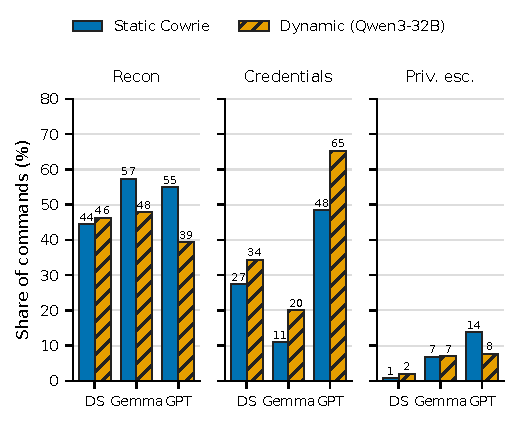
\includegraphics[width=\columnwidth]{fig_attackers}
\caption{Share of commands that match each keyword category, per attacker and honeypot backend. DS = DeepSeek-V3.2, Gemma = Gemma-3-4B, GPT = GPT-OSS-120B. Static: stock Cowrie. Dynamic: Cowrie backed by Qwen3-32B. A command can match several categories.}
\label{fig:attackers}
\end{figure}

\subsection{Attacker behavior and honeypot backends}\label{sec:behavior}

The three attackers behaved quite differently under the same prompt (Table~\ref{tab:cells}). On the static honeypot, DeepSeek-V3.2 ran the shortest sessions (13.5 turns on average) and Gemma-3-4B the longest (21.0). GPT-OSS-120B issued 280 unique commands, against 158 for Gemma-3-4B and 124 for DeepSeek-V3.2. It was also the most interested in secrets. Of its static-backend commands, 48.5\% matched our credential keywords, against 27.4\% for DeepSeek-V3.2 and 11.0\% for Gemma-3-4B. Its privilege-escalation share was 13.8\%, against 6.9\% for Gemma-3-4B and 0.7\% for DeepSeek-V3.2.

The LLM-backed honeypot pushed all three attackers toward credential hunting (Fig.~\ref{fig:attackers}). The credential share rose from 27.4\% to 34.4\% for DeepSeek-V3.2 and from 11.0\% to 20.0\% for Gemma-3-4B. For GPT-OSS-120B it rose from 48.5\% to 65.2\%. The dynamic backend was not uniformly slower. Mean latency fell by 17.1\% for DeepSeek-V3.2 and by 46.3\% for Gemma-3-4B, and it rose by 24.8\% for GPT-OSS-120B. Our latency is the time until the output goes quiet, so it also depends on which commands each attacker sent. We did not separate these effects.

Sessions also ended in different ways. DeepSeek-V3.2 finished on its own in 19 static and 20 dynamic sessions; it refused once. Gemma-3-4B reached the turn limit in 8 static sessions and timed out once. GPT-OSS-120B reached the turn limit in 17 of its 20 static sessions. On the dynamic backend it was the least stable attacker: 10 sessions lost the SSH connection, 6 ended with an LLM error, and only 4 completed. It never refused.

GPT-OSS-120B leaked chat-format tokens into the shell in 18 of its 40 sessions (11 static, 7 dynamic). These are control tokens from its own chat template, such as \cmd{\textless\textbar channel\textbar\textgreater analysis\textless\textbar message\textbar\textgreater}, followed by the model's private reasoning. Our harness treated the whole reply as a command and typed it into Cowrie. DeepSeek-V3.2 and Gemma-3-4B never did this. Left in place, the leaks would put long English sentences at a shell prompt and distort every statistic we report. We strip the tokens and the text after them. Some leaked text remains where the model joined commands with no separator.

\subsection{Synthetic versus real data without labels}\label{sec:shift}

\begin{figure}[t]
\centering
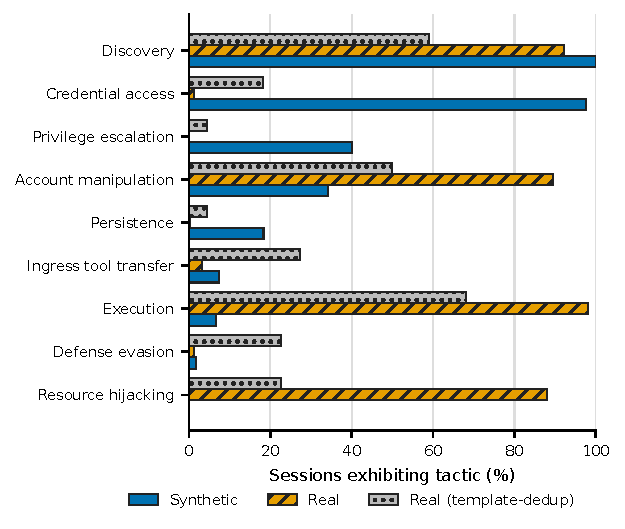
\includegraphics[width=\columnwidth]{fig_tactics}
\caption{Share of sessions that touch each ATT\&CK tactic at least once, for synthetic sessions (120), real sessions (1,672) and template-deduplicated real sessions (22).}
\label{fig:tactics}
\end{figure}

Real traffic is dominated by a few scripts, while every synthetic session is unique. The five most common templates cover 96.2\% of real interactive sessions but only 4.2\% of synthetic sessions. Real commands are also longer (53.3 against 43.0 characters on average) and more often chained (40.3\% against 19.4\%). Median session length is similar, at 23.0 real and 18.0 synthetic commands.

The largest real template alone covers 1,038 of the 1,672 sessions. It counts CPU cores, resets the root password with \cmd{chpasswd}, checks memory and the CPU model, and deletes old \cmd{dota} files. It then decodes and runs a base64-encoded shell script. The script unpacks a \cmd{dota.tar.gz} archive into a hidden directory under \cmd{/tmp}, starts an SSH scanner against private address ranges and runs the kit's setup script. This is consistent with what Trend Micro attributes to Outlaw~\cite{trendmicro2018outlaw}.

The tactic profiles barely overlap (Fig.~\ref{fig:tactics}). Every synthetic session touched discovery (100.0\%), and nearly all touched credential access (97.5\%). Many also probed privilege escalation (40.0\%) or persistence (18.3\%). In the real sessions, credential access, persistence and privilege escalation were almost absent, at 1.2\%, 0.4\% and 0.1\%. Real sessions instead touched execution (98.1\%), account manipulation (89.4\%) and resource hijacking (87.9\%). The synthetic shares for these were 6.7\%, 34.2\% and 0.0\%. Discovery is the one tactic both sides share, at 100.0\% against 92.2\%.

The template view is less extreme. Counted once per template, real discovery drops to 59.1\%, execution to 68.2\% and resource hijacking to 22.7\%. So the highest session-level shares come from a few heavily repeated scripts. Neither view looks like the synthetic profile.

The verb distributions are far apart. The JSD between synthetic and real verbs is 0.700 (95\% CI 0.688--0.717). Against template-deduplicated real data it is 0.729 (0.719--0.745). The two vocabularies share little, with a Jaccard index of 0.285. Yet the synthetic vocabulary covers 82.0\% of real verb occurrences. The agents know the commands; they use them in other proportions and for other purposes. The top synthetic verbs browse files: \cmd{ls} (712), \cmd{cat} (606), \cmd{head} (243) and \cmd{find} (217). The top real verbs process text and fingerprint the system: \cmd{grep} (8,880), \cmd{cat} (8,123), \cmd{echo} (6,964) and \cmd{uname} (4,437).

A simple classifier separates the two corpora almost perfectly. The C2ST AUC is 1.000~$\pm$~0.000 on normalized commands and 0.996~$\pm$~0.010 on verbs alone. The verb-only result shows that the separation does not depend on paths or arguments. Near-perfect separation does not prove that every downstream task will fail, but it is a strong warning.

\begin{figure}[t]
\centering
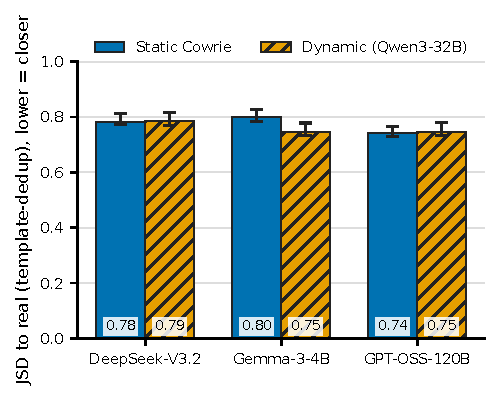
\includegraphics[width=\columnwidth]{fig_condition_jsd}
\caption{Verb-distribution JSD between each attacker--backend cell and template-deduplicated real traffic, with 95\% bootstrap confidence intervals. Lower values are closer to real traffic.}
\label{fig:jsd}
\end{figure}

All six attacker--backend cells stay far from real traffic (Fig.~\ref{fig:jsd}). Their JSD to template-deduplicated real data ranges from 0.741 to 0.798. Only Gemma-3-4B had a lower JSD on the dynamic backend (0.746 against 0.798), and only its intervals do not overlap. For DeepSeek-V3.2 (0.785 against 0.783) and GPT-OSS-120B (0.746 against 0.741), the dynamic value was slightly higher and the intervals overlap. The GPT-OSS-120B dynamic cell also ended differently, mostly in lost connections and LLM errors. For GPT-OSS-120B and Gemma-3-4B, the number of tactics whose presence or absence matches the real data rose from 5 to 7 of 9. We have 20 sessions per cell and made no correction for multiple comparisons, so no backend ordering is statistically established.

\subsection{Transfer between synthetic and real data}\label{sec:transfer}

\begin{table}[t]
\caption{Transfer results and final label counts. Labels come from blind dual-LLM annotation. Real labels are copied from 22 templates, so the effective real sample size is 22. Q2 and Q4 use GroupKFold by template. For Q1, Q2 and Q4, $n_{\mathrm{tr}}$ is the (mean) training size per fold and $n_{\mathrm{te}}$ counts pooled out-of-fold predictions. F1 is macro-F1 over the classes present in the test set. \lbl{Defense evasion} and \lbl{other} were never assigned.}
\label{tab:transfer}
\centering
\footnotesize
\setlength{\tabcolsep}{3pt}
(a) Transfer quadrants\\[3pt]
\begin{tabular}{@{}llrrcccc@{}}
\toprule
 & & & & \multicolumn{2}{c}{Classifier} & \multicolumn{2}{c}{Majority} \\
\cmidrule(lr){5-6}\cmidrule(lr){7-8}
Q & Train $\to$ test & $n_{\mathrm{tr}}$ & $n_{\mathrm{te}}$ & F1 & Acc. & F1 & Acc. \\
\midrule
Q1   & Syn $\to$ Syn          & 60    & 120   & 0.493 & 0.758 & 0.168 & 0.725 \\
Q2   & Real $\to$ Real        & 1,337 & 1,672 & 0.983 & 0.992 & 0.001 & 0.001 \\
Q3   & Syn $\to$ Real         & 120   & 1,672 & 0.205 & 0.022 & 0.000 & 0.000 \\
Q3-d & Syn $\to$ Real, dedup  & 120   & 22    & 0.071 & 0.045 & 0.000 & 0.000 \\
Q4   & Real+Syn $\to$ Real    & 1,457 & 1,672 & 0.981 & 0.992 & 0.001 & 0.001 \\
\bottomrule
\end{tabular}\\[8pt]
(b) Final label counts\\[3pt]
\begin{tabular}{@{}lrrr@{}}
\toprule
Label & Synthetic & Real sessions & Real templates \\
\midrule
\lbl{recon}                & 14  & 137   & 8 \\
\lbl{credential access}    & 87  & 0     & 0  \\
\lbl{privilege escalation} & 2   & 0     & 0  \\
\lbl{persistence}          & 11  & 443   & 5  \\
\lbl{malware drop}         & 6   & 52    & 6  \\
\lbl{resource hijacking}   & 0   & 1,040 & 3  \\
\midrule
Total                      & 120 & 1,672 & 22 \\
\bottomrule
\end{tabular}
\end{table}

The synthetic and real data have almost disjoint label sets (Table~\ref{tab:transfer}(b)). Synthetic sessions are mostly \lbl{credential access} (87 of 120). Real sessions are mostly \lbl{resource hijacking} (1,040) and \lbl{persistence} (443). \lbl{Resource hijacking} never occurs in the synthetic data. \lbl{Credential access} and \lbl{privilege escalation} never occur in the real data. The second-largest real template shows how thin some boundaries are. It runs the same fingerprinting steps as the dota dropper and changes a password with \cmd{passwd}. It never unpacks a payload, so it is labeled \lbl{persistence}.

The two annotators agreed well. Raw agreement was 0.935 and Cohen's kappa was 0.898 over all 184 items. Kappa was 0.873 on real items and 0.835 on synthetic items. The annotators agreed on 172 items, and the adjudicator resolved the other 12. The most frequent split was \lbl{recon} against \lbl{credential access}, on synthetic sessions that read sensitive files while exploring. One disagreement matters far more than the rest. On the dominant dota template, one annotator chose \lbl{malware drop} and the other chose \lbl{resource hijacking}. The adjudicator picked \lbl{resource hijacking}, following the rubric's tie-break. That single decision sets the label of 1,038 real sessions.

Real-to-real classification is easy, and synthetic-to-synthetic classification is moderate (Table~\ref{tab:transfer}(a)). Q1 reaches a macro-F1 of 0.493 and an accuracy of 0.758, above its majority baseline of 0.168 and 0.725. Q1 trains on only 60 sessions per fold, and two of its classes have 6 or fewer examples. Q2 reaches a macro-F1 of 0.983 and an accuracy of 0.992 on templates it never saw in training. We read Q2 as an upper bound. Near-duplicate scripts can still form separate templates in different folds, and real templates with the same label often share most of their commands.

The majority baseline for Q2 and Q4 is near zero (0.001) by construction. GroupKFold puts the whole dota template in one test fold, where the training majority is \lbl{persistence}. In the other folds the training majority is \lbl{resource hijacking}, which hardly occurs in their test sets.

Training on synthetic data alone fails on real data. Q3 reaches a macro-F1 of 0.205 and an accuracy of 0.022. With one session per template (Q3-dedup), the figures are 0.071 and 0.045. The model labels 1,636 of the 1,672 real sessions as \lbl{credential access}, the synthetic majority class, which never occurs in the real labels. The only class it recognizes is \lbl{malware drop}, with a per-class F1 of 0.818. Every other class scores 0.000, so the whole macro-F1 comes from that one class. The majority baseline scores 0.000 for the same reason: it always predicts \lbl{credential access}.

Adding synthetic data to the real training data gave no gain. Q4 reaches a macro-F1 of 0.981 against 0.983 for Q2, with the same accuracy (0.992).

To test whether the dota label drives these results, we reran the experiment with all three \lbl{resource hijacking} templates, including dota, labeled \lbl{malware drop}. Q3 stayed near zero (macro-F1 0.021), while Q2 and Q4 reached 0.933 and 0.965. The transfer failure does not depend on this label, and adding synthetic data gives no consistent benefit.

With labels from our keyword rules, Q3 also collapsed (macro-F1 0.000). We do not count this as evidence, because those labels share keywords with the features.

%% =====================================================================
\section{Discussion}\label{sec:discussion}

\subsection{The gap is about intent}
Our agents did not fail at their task; they did a different one. Asked to act like a curious intruder, they listed directories, read configuration files and searched for keys. The real traffic on our sample day came mostly from bots. They profiled the CPU, took over the account and launched a scanner and miner kit~\cite{trendmicro2018outlaw}. Nobody asked the agents to act like the dominant real population.

\subsection{What the transfer result means}
The Q3 failure is first a label-space problem. With no \lbl{resource hijacking} sessions, a synthetic-trained model cannot predict the label of most real sessions. But \lbl{recon} and \lbl{persistence}, which both corpora contain, also score an F1 of 0.000. Synthetic persistence is an intruder writing a reverse-shell cron entry or appending an SSH key. Real persistence is a bot script that changes a password between fingerprinting steps. The label is the same; the behavior is not. In our setting, more sessions from the same persona are unlikely to close this gap.

\subsection{The LLM-backed honeypot}
Qwen3-32B lowered the divergence only for Gemma-3-4B, the smallest attacker. Richer shell output may give a weak attacker more to react to; we have not tested this. Even the closest cell (JSD 0.741) is far from real traffic. The backend also raised the share of credential-hunting commands for every attacker. Credential access is exactly the intent that never appears in our real labels.

\subsection{Leakage and next steps}
A harness that treats the model's reply as the literal action will type leaked control tokens and reasoning into the terminal. The transcript still looks like a session, but much of it is the model thinking aloud. Pipelines should screen each command for known control tokens and log the raw reply apart from the executed command. Future work should try bot-like personas (dropper, cryptominer, credential stuffer). Work on synthetic honeypot data should also report label-free shift measures next to classifier scores.

%% =====================================================================
\section{Threats to Validity}\label{sec:threats}

Our labels come from LLMs, and we did not validate them against human annotators. Both annotators and the adjudicator are Claude models from one provider, and they may share biases. Their high agreement (kappa 0.898) may therefore overstate how correct the labels are. The most consequential label, for the dota template, was set by the adjudicator after a split; changing it leaves Q3 near zero (Section~\ref{sec:transfer}). A human audit of all 184 items is future work. We release the full annotation kit so that others can run it: the rubric, the blinded sheets, both annotators' labels and the adjudicator's rationales.

Blindness is imperfect. The annotators never saw an item's source, but LLM-generated commands have a recognizable style, with clean single commands and tidy flags. An annotator may guess the source and be swayed by it. We cannot measure how often this happened.

The synthetic sample is small, with 20 sessions per attacker--backend cell and no correction for multiple comparisons.

The real data cover one day (2019-11-15) of one honeynet. One campaign dominates, the top five templates cover 96.2\% of interactive sessions, and the effective real sample is only 22 templates. Template-level results soften the dominance, but deduplication has its own effect: it raises the JSD from 0.700 to 0.729.

The tactic tagger and the keyword shares in Table~\ref{tab:cells} use regular expressions that we wrote. They can mislabel commands; for example, any path that contains \cmd{passwd} looks like credential access. Differences as large as those in Fig.~\ref{fig:tactics} are unlikely to be tagger artifacts, but small ones may be.

All sessions use one prompt, three attacker models and one backend model, so persona effects are not separated from model effects. Our conclusions concern these models under this persona, not LLM attackers in general. Last, leak stripping cannot repair glued commands, and the C2ST uses a single classifier family. A perfect AUC shows that the corpora are separable, not that no other representation could bridge them.

%% =====================================================================
\section{Ethics}

The attacker agents targeted only our own isolated honeypot. It holds no real data and has no route to third-party systems. The harness takes one explicit target and has no scanning or discovery features. The real data are the public CyberLab release under CC~BY~4.0, in which source IP addresses are replaced by hashes. We made no attempt to re-identify any source. We used only session IDs, event timestamps and command text, and the LLM annotators saw only command transcripts. The released code adds no attack capability beyond standard post-compromise commands that already appear in public honeypot data.

%% =====================================================================
\section{Conclusion}

We asked whether LLM red-team agents produce honeypot traffic that is realistic enough to train defenses for real traffic. Under one ``explore the system'' persona, the answer in our setting is no. Our 120 synthetic sessions sit far from a day of real CyberLab sessions (JSD 0.700), and a simple classifier separates them perfectly (AUC 1.000). The agents browse files and hunt for credentials, while most real sessions run one cryptominer dropper. A classifier trained on these synthetic sessions reaches a macro-F1 of 0.205 on real sessions, against 0.983 for one trained on real data. Adding synthetic data gives no gain (0.981). The LLM-backed honeypot lowered the divergence only for Gemma-3-4B, and every cell stayed far from real traffic. These results rest on a small synthetic corpus, one day of 2019 data with 22 real behavior templates, one persona and LLM-made labels. Next, we plan personas aimed at the bot population, more days and honeynets, and a human audit of the labels. Contamination checks such as the chat-format leak rate should become standard reporting for synthetic honeypot data.

\section*{Code and Data Availability}

We release the attacker harness, the CyberLab parser, the normalization and tagging module, and the scripts that produce every table and figure. The release also contains the annotation kit with both annotators' labels and the adjudication rationales. The real data are available on Zenodo at \url{https://doi.org/10.5281/zenodo.3687527}~\cite{sedlar2020cyberlab}. Every number in this paper is written to a results file by one of the released scripts.

{\sloppy
\bibliographystyle{IEEEtran}
\bibliography{references}}

\end{document}
